%%%
% Plantilla de Memoria
% Modificación de una plantilla de Latex de Nicolas Diaz para adaptarla 
% al castellano y a las necesidades de escribir informática y matemáticas.
%
% Editada por: Mario Román
%
% License:
% CC BY-NC-SA 3.0 (http://creativecommons.org/licenses/by-nc-sa/3.0/)
%%%

%%%%%%%%%%%%%%%%%%%%%%%%%%%%%%%%%%%%%%%%%
% Thin Sectioned Essay
% LaTeX Template
% Version 1.0 (3/8/13)
%
% This template has been downloaded from:
% http://www.LaTeXTemplates.com
%
% Original Author:
% Nicolas Diaz (nsdiaz@uc.cl) with extensive modifications by:
% Vel (vel@latextemplates.com)
%
% License:
% CC BY-NC-SA 3.0 (http://creativecommons.org/licenses/by-nc-sa/3.0/)
%
%%%%%%%%%%%%%%%%%%%%%%%%%%%%%%%%%%%%%%%%%

%----------------------------------------------------------------------------------------
%	PAQUETES Y CONFIGURACIÓN DEL DOCUMENTO
%----------------------------------------------------------------------------------------

%%% Configuración del papel.
% microtype: Tipografía.
% mathpazo: Usa la fuente Palatino.
\documentclass[a4paper, 17pt]{article}
%\usepackage[a4paper,margin=1in,footskip=1in]{geometry}
\usepackage[protrusion=true,expansion=true]{microtype}
\usepackage{mathpazo}

% Indentación de párrafos para Palatino
\setlength{\parindent}{0pt}
  \parskip=8pt
\linespread{1.05} % Change line spacing here, Palatino benefits from a slight increase by default


%%% Castellano.
% noquoting: Permite uso de comillas no españolas.
% lcroman: Permite la enumeración con numerales romanos en minúscula.
% fontenc: Usa la fuente completa para que pueda copiarse correctamente del pdf.
\usepackage[spanish,es-noquoting,es-lcroman,es-tabla]{babel}
\usepackage[utf8]{inputenc}
\usepackage[T1]{fontenc}
\selectlanguage{spanish}


%%% Gráficos
\usepackage{graphicx} % Required for including pictures
\usepackage{wrapfig} % Allows in-line images
\usepackage[usenames,dvipsnames]{color} % Coloring code
\graphicspath{{./Capturas/}}

%%% Matemáticas
\usepackage{amsmath}

%%% Pseudocódigo
\usepackage{algorithmicx}
\usepackage[ruled]{algorithm}
\usepackage{algpseudocode}

\newcommand{\alg}{\texttt{algorithmicx}}
\newcommand{\old}{\texttt{algorithmic}}
\newcommand{\euk}{Euclid}
\newcommand\ASTART{\bigskip\noindent\begin{minipage}[b]{0.5\linewidth}}
\newcommand\ACONTINUE{\end{minipage}\begin{minipage}[b]{0.5\linewidth}}
\newcommand\AENDSKIP{\end{minipage}\bigskip}
\newcommand\AEND{\end{minipage}}

%%% Código
\usepackage{listings}

%%% Tablas
\usepackage{tabularx}
\usepackage{float}
\usepackage{adjustbox}
\usepackage{booktabs}

%%% Bibliografía
\makeatletter
\renewcommand\@biblabel[1]{\textbf{#1.}} % Change the square brackets for each bibliography item from '[1]' to '1.'
\renewcommand{\@listI}{\itemsep=0pt} % Reduce the space between items in the itemize and enumerate environments and the bibliography

%----------------------------------------------------------------------------------------
%	TÍTULO
%----------------------------------------------------------------------------------------
% Configuraciones para el título.
% El título no debe editarse aquí.
\renewcommand{\maketitle}{
  \begin{flushright} % Right align
  
  {\LARGE\@title} % Increase the font size of the title
  
  \vspace{50pt} % Some vertical space between the title and author name
  
  {\large\@author} % Author name
  \\\@date % Date
  \vspace{40pt} % Some vertical space between the author block and abstract
  \end{flushright}
}

%% Título
\title{\textbf{Título}\\ % Title
Subtítulo} % Subtitle

\author{\textsc{Autor1,\\Autor2} % Author
\\{\textit{Universidad de Granada}}} % Institution

\date{\today} % Date

%-----------------------------------------------------------------------------------------
%	DOCUMENTO
%-----------------------------------------------------------------------------------------

\begin{document}

%-----------------------------------------------------------------------------------------
%	TITLE PAGE
%-----------------------------------------------------------------------------------------

\begin{titlepage} % Suppresses displaying the page number on the title page and the subsequent page counts as page 1
	
	\raggedleft % Right align the title page
	
	\rule{1pt}{\textheight} % Vertical line
	\hspace{0.05\textwidth} % Whitespace between the vertical line and title page text
	\parbox[b]{0.75\textwidth}{ % Paragraph box for holding the title page text, adjust the width to move the title page left or right on the page
		
		{\Huge\bfseries Práctica 1:\\[0.5\baselineskip] Análisis Predictivo Empresarial Mediante Clasificación}\\[2\baselineskip] % Title
		{\large\textit{Curso 2019/2020}}\\[4\baselineskip] % Subtitle or further description
		{\Large\textsc{Sofía Almeida Bruno}\\[0.5\baselineskip]sofialmeida@correo.ugr.es} % Author name, lower case for consistent small caps
		
		\vspace{0.4\textheight} % Whitespace between the title block and the publisher
		
		{\noindent Grupo IN 2\\[0.5\baselineskip] Jueves 9:30-10:30}\\[\baselineskip] % Publisher and logo
	}

\end{titlepage}

%% Resumen (Descomentar para usarlo)
%\renewcommand{\abstractname}{Resumen} % Uncomment to change the name of the abstract to something else
%\begin{abstract}
% Resumen aquí
%\end{abstract}

%% Palabras clave
%\hspace*{3,6mm}\textit{Keywords:} lorem , ipsum , dolor , sit amet , lectus % Keywords
%\vspace{30pt} % Some vertical space between the abstract and first section


%% Índice
{\parskip=2pt
  \tableofcontents
}
\pagebreak

%%% Inicio del documento
%%%%%%%%%%%%%%%%%%%%%%%%%%%%%%%%%%%%%%%%%%%%%%%%%%%%%%%%%%%%%%%%%%%
%       DESCRIPCIÓN DEL PROBLEMA
%%%%%%%%%%%%%%%%%%%%%%%%%%%%%%%%%%%%%%%%%%%%%%%%%%%%%%%%%%%%%%%%%%%
\section{Introducción}

En este práctica se abordará un problema de clasificación del mundo real para, mediante el uso de los algoritmos de clasificación supervisada vistos en clase de teoría y las herramientas y recursos expuestos en clase de prácticas, realizar una predicción sobre el mismo y analizar cómo de buena es esta clasificación. Se compararán distintos algoritmos y se examinará la predicción obtenida en función a los mismos según distintos criterios de precisión.

El problema con el que se trabajará proviene de la plataforma ``Driven data'', usa los datos de ``Taarifa'' (API web libre que está trabajando en un poryecto de innovación en Tanzania) y del Ministerio de Agua de Tanzania. El objetivo es predecir qué bombas de agua funcionan, cuáles necesitan alguna reparación y cuáles están rotas. Es decir, estamos ante un problema de clasificación con tres clases diferentes. Se trata de predecir mediante variables como: qué tipo de bomba es, cuándo se instaló, cantidad de agua disponible,... ante qué tipo de bomba de agua nos encontramos. Saber qué puntos de agua fallarán permitirá mejorar las tareas de mantenimiento y asegurar que hay agua limpia y potable disponible para las comunidades de Tanzania.

Abordaremos el problema a partir de un conjunto de datos formado por 59.400 instancias, de las cuales conocemos información sobre 39 variables, además de su clase (una de las tres ya mencionadas).
Usando el nodo \texttt{Data Explorer} podemos hacer una exploración inicial del conjunto. En primer lugar, observamos la frecuencia de las clases: de todas las instancias 32259 son bombas de agua funcionales, 22824 no funcionales y 4317 funcionales pero necesitan una reparación. Las clases están desbalanceadas, observamos una gran diferencia en el número de ejemplos de bombas funcionales y aquellas que pese a ser funcionales requieren mantenimiento.

Nada más cargar el fichero observamos que es un conjunto de datos que posee valores perdidos, además de algunos valores ``unknown''. 

Toda la experimentación se realizará usando una validación cruzada de 5 particiones. La semilla aleatoria empleada en aquellos algoritmos que lo requieran será: 12345.
Los experimentos realizados en esta práctica se ejecutaron en un ordenador con sistema operativo Ubuntu 16.04 con procesador Intel(R) Core(TM) i5-2410M CPU @ 2.30GHz.

Se utilizará la validación cruzada en la ejecución de todos los algoritmos, mediante los nodos \texttt{X-Partitioner} y \texttt{X-Aggregator} de KNIME. Se configuran para crear 5 particiones, luego en cada experimento se utilizará un conjunto de entrenamiento de tamaño 47520 y un conjunto de prueba formado por 11.880 instancias.

Hemos visto en clase que comparar los algoritmos solo por la precisión que consiguen en la predicción no es suficiente, ya que en conjuntos desbalanceados malos algoritmos podrían obtener una alta precisión. Así, utilizaremos medidas sensibles al desbalanceo. Se siguió el tutorial proporcionado por el profesor de prácticas sobre cómo comparar diferentes algoritmos para obtener las tablas de resultados.
%%%%%%%%%%%%%%%%%%%%%%%%%%%%%%%%%%%%%%%%%%%%%%%%%%%%%%%%%%%%%%%%%%%
%       EXPERIMENTOS Y ANÁLISIS DE RESULTADOS
%%%%%%%%%%%%%%%%%%%%%%%%%%%%%%%%%%%%%%%%%%%%%%%%%%%%%%%%%%%%%%%%%%%
\section{Resultados obtenidos}
%%%%%%%%%%%%%%%%%%%%%%%%%%%%%%%%%%%%%%%%%
%%%%%%%       ZeroR
%%%%%%%%%%%%%%%%%%%%%%%%%%%%%%%%%%%%%%%%%
\section{ZeroR}
Para comenzar (y sin incluirlo como algoritmo a estudiar), he decidido observar el comportamiento del clasificador ZeroR. Este clasificador predice que cualquier instancia pertenecerá a la clase mayoritaria. Aunque ya sabemos que no obtendremos un buen resultado utilizando este clasificador porque solo clasificará correctamente las instancias que verdaderamente pertenezcan a la clase mayoritaria, nos servirá para tener una cota inferior de las medidas. Si en algún momento durante el desarrollo de la práctica obtuvieramos resultados peores que los obtenidos con este clasificador sospecharemos que estamos haciendo algo mal.

Podemos observar el metanodo creado en KNIME para este algoritmo en la Figura \ref{fig:zeroR}. Se ha utilizado el nodo \texttt{ZeroR} de \texttt{Weka}.

\begin{figure}[H]
    \centering
    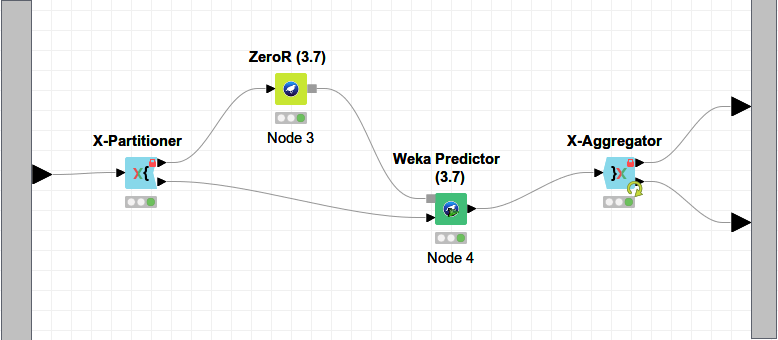
\includegraphics[width=1\textwidth]{ZeroR}
    \caption{Metanodo ZeroR}
    \label{fig:zeroR}
\end{figure}

En la Tabla \ref{tab:zeroR} se encuentran las medidas de precisión obtenidas con este algoritmo. En este caso, conociendo la distribución de las clases, se podrían haber calculado manualmente sin necesidad de ejecutar el algoritmo, pues por su naturaleza el número de verdaderos positivos (TP) se corresponderá al número 

\begin{table}[H]
  \label{tab:zeroR}
  \centering
  \caption{ZeroR - criterios de precisión}
  \begin{tabular}{lrrrrrrrrrr}
    \toprule
    & TP & FP & TN & FN & TPR & TNR & PPV & Accur. & F1-score & G-mean\\ \midrule
    ZeroR & 32259 & 27414 & 0 & 0 & 1 & 0 & 0.543 & 0.543 & 0.704 & 0 \\
    \bottomrule
  \end{tabular}
\end{table}



\subsection{C4.5}



\subsection{Resultados obtenidos}
\subsubsection{1-NN}
\begin{table}[H]
  \centering
  \caption{Colposcopy}
  \begin{tabular}{lrrrr}
    \toprule
    & Tasa clasificación & Tasa reducción & Agregado & Tiempo ($\mu s$)\\ \midrule
    Partición 1 & 74.5763 & 0 & 37.2881 & 4316 \\
    Partición 2 & 70.1754 & 0 & 35.0877 & 3613 \\
    Partición 3 & 73.6842 & 0 & 36.8421 & 5636 \\
    Partición 4 & 75.4386 & 0 & 37.7193 & 3638 \\
    Partición 5 & 82.4561 & 0 & 41.2281 & 3411 \\
    \midrule
    Media & 75.2661 & 0 & 37.6331 & 4122.8 \\
    \bottomrule
  \end{tabular}

  \bigskip
  \caption{Ionosphere}
  \begin{tabular}{lrrrr}
    \toprule
    & Tasa clasificación & Tasa reducción & Agregado & Tiempo ($\mu s$)\\ \midrule
    Partición 1 & 90.1408 & 0 & 45.0704 & 3804 \\
    Partición 2 & 80 & 0 & 40 & 3470 \\
    Partición 3 & 82.8571 & 0 & 41.4286 & 3319 \\
    Partición 4 & 92.8571 & 0 & 46.4286 & 3938 \\
    Partición 5 & 87.1429 & 0 & 43.5714 & 3443 \\
    \midrule
    Media & 86.5996 & 0 & 43.2998 & 3594.8 \\
    \bottomrule
  \end{tabular}

  \bigskip
  \caption{Texture}
  \begin{tabular}{lrrrr}
    \toprule
    & Tasa clasificación & Tasa reducción & Agregado & Tiempo ($\mu s$)\\ \midrule
    Partición 1 & 93.6364 & 0 & 46.8182 & 9351 \\
    Partición 2 & 89.0909 & 0 & 44.5455 & 8895 \\
    Partición 3 & 94.5455 & 0 & 47.2727 & 8251 \\
    Partición 4 & 92.7273 & 0 & 46.3636 & 7658 \\
    Partición 5 & 92.7273 & 0 & 46.3636 & 7524 \\
    \midrule
    Media & 92.5455 & 0 & 46.2727 & 8335.8 \\
    \bottomrule
  \end{tabular}
\end{table}

\subsubsection{Resultados globales}
\begin{table}[H]
  \centering
  \caption{Colposcopy}
  \begin{tabular}{lrrrr}
    \toprule
    Algoritmo & Tasa clasificación & Tasa reducción & Agregado & Tiempo ($\mu s$)\\ \midrule
    1-NN & 75.2661 & 0 & 37.6331 & 4122.8 \\
    RELIEF & 75.9798 & 36.4516 & 56.2157 & 12357.8 \\
    BL & 76.2831 & 14.5161 & 45.3996 & 7.07349e+06 \\
    \bottomrule
  \end{tabular}

  \bigskip
  \caption{Ionosphere}
  \begin{tabular}{lrrrr}
    \toprule
    Algoritmo & Tasa clasificación & Tasa reducción & Agregado & Tiempo ($\mu s$)\\ \midrule
    1-NN & 86.5996 & 0 & 43.2998 & 3594.8 \\
    RELIEF & 87.4567 & 2.94118 & 45.199 & 10962.6 \\
    BL & 86.0402 & 20.5882 & 53.3142 & 5.62155e+06 \\
    \bottomrule
  \end{tabular}

  \bigskip
  \caption{Texture}
  \begin{tabular}{lrrrr}
    \toprule
    Algoritmo & Tasa clasificación & Tasa reducción & Agregado & Tiempo ($\mu s$)\\ \midrule
    1-NN & 92.5455 & 0 & 46.2727 & 8335.8 \\
    RELIEF & 93.0909 & 5.5 & 49.2955 & 19242.4 \\
    BL & 90.7273 & 22.5 & 56.6136 & 1.40398e+07 \\
    \bottomrule
  \end{tabular}
\end{table}

\section{Análisis de resultados}


\section{Configuración de algoritmos}

\section{Procesado de datos}

\section{Interpretación de resultados}

\section{Contenido adicional}
%%%%%%%%%%%%%%%%%%%%%%%%%%%%%%%%%%%%%%%%%%%%%%%%%%%%%%%%%%%%%%%%%%%
%       REFERENCIAS
%%%%%%%%%%%%%%%%%%%%%%%%%%%%%%%%%%%%%%%%%%%%%%%%%%%%%%%%%%%%%%%%%%%
\section{Bibliografía}
\end{document}
